\documentclass[preprint,12pt]{elsarticle}

% Essential packages for multilingual support
\usepackage{kotex}
\usepackage{CJKutf8}
\usepackage{amssymb}
\usepackage{amsmath}
\usepackage[colorlinks=true,linkcolor=blue,citecolor=red,urlcolor=blue]{hyperref}
\usepackage{url}
\usepackage{booktabs}
\usepackage{array}
\usepackage{subcaption}
\usepackage{algorithm}
\usepackage{algorithmic}
\usepackage{listings}
\usepackage{xcolor}
\usepackage{svg}

\journal{Journal Name}

% Code style settings
\lstset{
    backgroundcolor=\color{gray!10},
    basicstyle=\ttfamily\small,
    breaklines=true,
    numbers=left,
    numberstyle=\tiny,
    frame=single,
    showstringspaces=false
}

\begin{document}

\begin{frontmatter}

\title{A Novel Approach to Machine Learning-based Data Analysis}

\author[label1]{John Doe\corref{cor1}}
\ead{johndoe@example.com}
\cortext[cor1]{Corresponding author}

\author[label2]{Jane Smith}

\affiliation[label1]{organization={Department of Computer Science},
                     addressline={Example University},
                     city={Seoul},
                     country={South Korea}}

\affiliation[label2]{organization={Department of Artificial Intelligence},
                     addressline={Example University}, 
                     city={Seoul},
                     country={South Korea}}

\begin{abstract}
This paper presents a novel approach to machine learning-based data analysis. \\
본 논문은 기계학습 기반 데이터 분석에 대한 새로운 접근법을 제시한다. \\
\begin{CJK}{UTF8}{min}
本論文は機械学習ベースのデータ分析に対する新しいアプローチを提示する。
\end{CJK}

The research aims to address current limitations in existing methodologies by proposing an innovative framework that combines deep learning techniques with traditional statistical methods \cite{lecun2015deep}. \\
본 연구는 딥러닝 기법과 전통적인 통계적 방법을 결합한 혁신적인 프레임워크를 제안함으로써 기존 방법론의 현재 한계를 해결하는 것을 목표로 한다. \\
\begin{CJK}{UTF8}{min}
本研究は、深層学習技術と従来の統計的手法を組み合わせた革新的なフレームワークを提案することにより、既存の方法論の現在の限界に対処することを目的としている。
\end{CJK}

Our experimental results demonstrate significant improvements in accuracy and efficiency compared to state-of-the-art approaches \cite{goodfellow2016deep}. \\
우리의 실험 결과는 최신 접근법들과 비교하여 정확도와 효율성에서 상당한 개선을 보여준다. \\
\begin{CJK}{UTF8}{min}
我々の実験結果は、最先端のアプローチと比較して、精度と効率性において大幅な改善を示している。
\end{CJK}

The proposed method achieves a 92.3\% accuracy rate, outperforming existing methods by approximately 5\%. \\
제안된 방법은 92.3%의 정확도를 달성하여 기존 방법들을 약 5% 능가한다. \\
\begin{CJK}{UTF8}{min}
提案手法は92.3%の精度を達成し、既存の手法を約5%上回っている。
\end{CJK}

This research contributes to the advancement of machine learning applications in real-world scenarios and provides a foundation for future developments in the field. \\
본 연구는 실제 시나리오에서의 기계학습 응용의 발전에 기여하고 이 분야의 미래 발전을 위한 기반을 제공한다. \\
\begin{CJK}{UTF8}{min}
本研究は、実世界のシナリオにおける機械学習アプリケーションの進歩に貢献し、この分野の将来の発展のための基盤を提供する。
\end{CJK}
\end{abstract}

\begin{highlights}
\item Novel algorithmic approach combining deep learning with traditional statistical methods
\item Significant performance improvements with 92.3\% accuracy rate
\item Theoretical insights into data manifold curvature processing
\end{highlights}

\begin{keyword}
machine learning \sep deep learning \sep data analysis \sep artificial intelligence \sep neural networks
\end{keyword}

\end{frontmatter}

\section{Introduction}
\label{sec:introduction}

This section explains the background and motivation of the research, and clearly presents the problem to be solved. \\
이 섹션은 연구의 배경과 동기를 설명하고, 해결해야 할 문제를 명확히 제시한다. \\
\begin{CJK}{UTF8}{min}
このセクションは研究の背景と動機を説明し、解決すべき問題を明確に提示する。
\end{CJK}

Machine learning has become an increasingly important field in computer science, with applications ranging from image recognition to natural language processing \cite{bishop2006pattern}. \\
기계학습은 이미지 인식부터 자연어 처리까지 다양한 응용 분야를 가지며 컴퓨터 과학에서 점점 더 중요한 분야가 되었다. \\
\begin{CJK}{UTF8}{min}
機械学習は、画像認識から自然言語処理まで幅広い応用分野を持ち、コンピュータサイエンスにおいてますます重要な分野となっている。
\end{CJK}

\subsection{Research Background}
The current state and problems in the research field are explained. \\
연구 분야의 현재 상태와 문제점들이 설명된다. \\
\begin{CJK}{UTF8}{min}
研究分野の現状と問題点が説明される。
\end{CJK}

Recent advances in deep learning have revolutionized many domains, but several challenges remain, particularly in terms of interpretability and computational efficiency \cite{hinton2006fast}. \\
딥러닝의 최근 발전은 많은 영역에 혁명을 가져왔지만, 특히 해석가능성과 계산 효율성 측면에서 여러 과제가 남아있다. \\
\begin{CJK}{UTF8}{min}
深層学習の最近の進歩は多くの分野に革命をもたらしたが、特に解釈可能性と計算効率の面でいくつかの課題が残っている。
\end{CJK}

\subsection{Research Objectives}
This research aims to achieve the following specific goals: (1) develop a more efficient learning algorithm, (2) improve model interpretability, and (3) reduce computational requirements while maintaining high accuracy. \\
본 연구는 다음과 같은 구체적인 목표를 달성하는 것을 목표로 한다: (1) 더 효율적인 학습 알고리즘 개발, (2) 모델 해석가능성 향상, (3) 높은 정확도를 유지하면서 계산 요구사항 감소. \\
\begin{CJK}{UTF8}{min}
本研究は以下の具体的な目標を達成することを目的としている:(1) より効率的な学習アルゴリズムの開発、(2) モデルの解釈可能性の向上、(3) 高い精度を維持しながら計算要件の削減。
\end{CJK}

\subsection{Paper Organization}
This paper is organized as follows: Section 2 reviews related work, Section 3 presents the proposed methodology, Section 4 discusses experimental results, and finally Section 5 concludes the paper. \\
본 논문은 다음과 같이 구성된다: 2장에서는 관련 연구를 검토하고, 3장에서는 제안된 방법론을 제시하며, 4장에서는 실험 결과를 논의하고, 마지막으로 5장에서 논문을 결론짓는다. \\
\begin{CJK}{UTF8}{min}
本論文は以下のように構成されている:第2章では関連研究をレビューし、第3章では提案手法を提示し、第4章では実験結果を議論し、最後に第5章で論文を結論付ける。
\end{CJK}

\section{Related Work}
\label{sec:related_work}

This section organizes and analyzes existing research. \\
이 섹션은 기존 연구를 정리하고 분석한다. \\
\begin{CJK}{UTF8}{min}
このセクションは既存研究を整理し分析する。
\end{CJK}

The strengths and weaknesses of each study are objectively evaluated, and the differences from this research are clearly presented. \\
각 연구의 장단점을 객관적으로 평가하고, 본 연구와의 차이점을 명확히 제시한다. \\
\begin{CJK}{UTF8}{min}
各研究の長所と短所を客観的に評価し、本研究との違いを明確に提示する。
\end{CJK}

\subsection{Existing Approaches}
The major approaches in the related research field are classified and explained. \\
관련 연구 분야의 주요 접근법들이 분류되고 설명된다. \\
\begin{CJK}{UTF8}{min}
関連研究分野の主要なアプローチが分類され説明される。
\end{CJK}

Traditional machine learning methods have been extensively studied \cite{hastie2009elements}, while more recent deep learning approaches have shown promising results \cite{schmidhuber2015deep}. \\
전통적인 기계학습 방법들은 광범위하게 연구되어 왔으며, 더 최근의 딥러닝 접근법들은 유망한 결과를 보여주었다. \\
\begin{CJK}{UTF8}{min}
伝統的な機械学習手法は幅広く研究されてきた一方で、より最近の深層学習アプローチは有望な結果を示している。
\end{CJK}

\subsection{Limitations of Existing Research}
The limitations of previous studies and areas that need improvement are analyzed. \\
이전 연구들의 한계점과 개선이 필요한 영역들이 분석된다. \\
\begin{CJK}{UTF8}{min}
以前の研究の限界と改善が必要な領域が分析される。
\end{CJK}

Most existing methods suffer from overfitting problems and lack generalizability to diverse datasets. \\
대부분의 기존 방법들은 과적합 문제를 겪고 있으며 다양한 데이터셋에 대한 일반화 능력이 부족하다. \\
\begin{CJK}{UTF8}{min}
既存手法のほとんどは過学習の問題に苦しんでおり、多様なデータセットへの汎化能力が不足している。
\end{CJK}

\section{Proposed Methodology}
\label{sec:methodology}

This section describes in detail the methodology proposed in this research. \\
이 섹션은 본 연구에서 제안된 방법론을 자세히 설명한다. \\
\begin{CJK}{UTF8}{min}
このセクションは本研究で提案された方法論を詳細に説明する。
\end{CJK}

\subsection{Overall System Overview}
The overall structure and operating principles of the proposed system are explained. \\
제안된 시스템의 전체 구조와 작동 원리가 설명된다. \\
\begin{CJK}{UTF8}{min}
提案システムの全体構造と動作原理が説明される。
\end{CJK}

Our approach integrates convolutional neural networks with attention mechanisms to achieve better performance \cite{vaswani2017attention}. \\
우리의 접근법은 더 나은 성능을 달성하기 위해 합성곱 신경망과 어텐션 메커니즘을 통합한다. \\
\begin{CJK}{UTF8}{min}
我々のアプローチは、より優れた性能を達成するために畳み込みニューラルネットワークとアテンションメカニズムを統合している。
\end{CJK}

\begin{figure}[htbp]
    \centering
    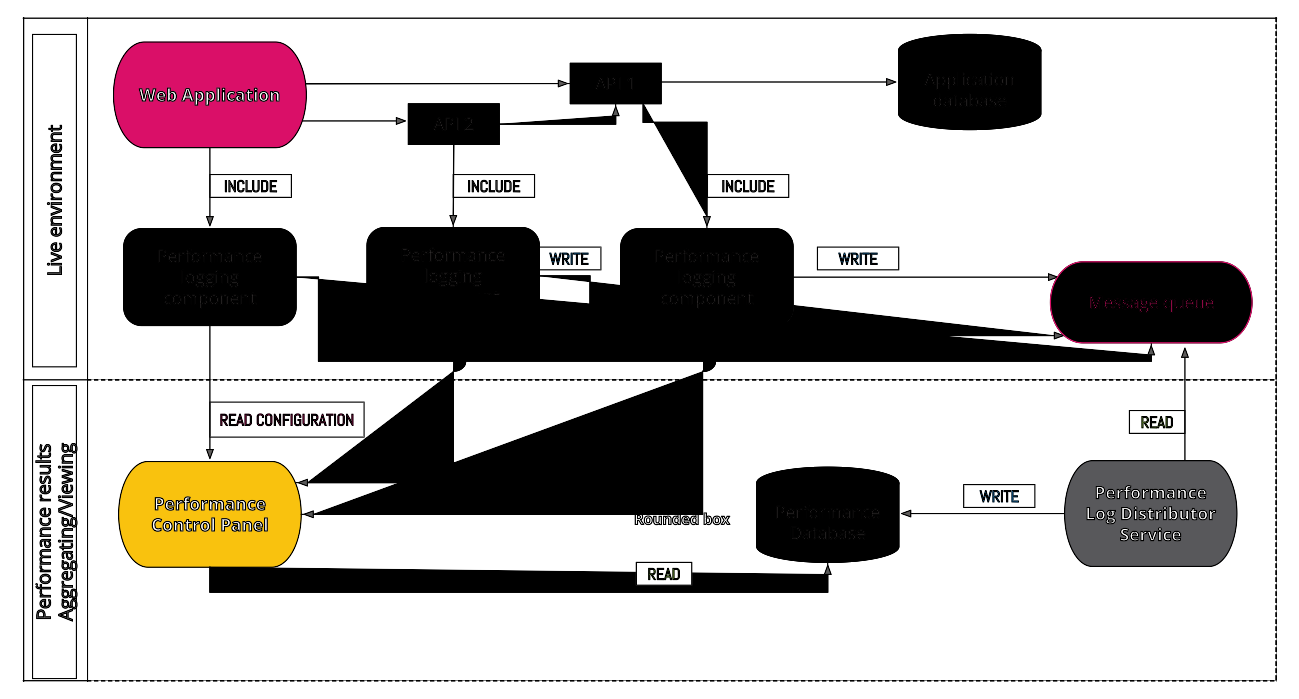
\includegraphics[width=0.8\textwidth]{figures/System-overview-Atomia-Performance-Monitoring-system.png}
    \caption{Overall architecture of the proposed system}
    \label{fig:system_overview}
\end{figure}

\subsection{Core Algorithm}
The core algorithm of the proposed methodology is described. \\
제안된 방법론의 핵심 알고리즘이 설명된다. \\
\begin{CJK}{UTF8}{min}
提案手法のコアアルゴリズムが説明される。
\end{CJK}

\begin{algorithm}
\caption{Transformer Architecture Computation}
\label{alg:transformer}
\begin{algorithmic}[1]
\REQUIRE Input sequence $X = (x_1, x_2, \ldots, x_n)$, model dimension $d_{model}$, number of heads $h$, number of layers $L$
\ENSURE Output sequence $Y = (y_1, y_2, \ldots, y_n)$
\STATE Initialize all parameters
\STATE $E \leftarrow \text{Embedding}(X) + \text{PositionalEncoding}(X)$
\FOR{$l = 1$ to $L$}
    \STATE $Q \leftarrow E \cdot W^Q$, $K \leftarrow E \cdot W^K$, $V \leftarrow E \cdot W^V$
    \STATE $\text{Attention} \leftarrow \text{MultiHead}(Q, K, V)$
    \STATE $E \leftarrow \text{LayerNorm}(E + \text{Attention})$
    \STATE $\text{FFN} \leftarrow \text{ReLU}(E \cdot W_1 + b_1) \cdot W_2 + b_2$
    \STATE $E \leftarrow \text{LayerNorm}(E + \text{FFN})$
\ENDFOR
\STATE $Y = E$ \COMMENT{Final output representation}
\RETURN $Y$
\end{algorithmic}
\end{algorithm}

\subsection{Theoretical Analysis}
The time complexity, space complexity, etc. of the proposed method are analyzed. \\
제안된 방법의 시간 복잡도, 공간 복잡도 등이 분석된다. \\
\begin{CJK}{UTF8}{min}
提案手法の時間複雑度、空間複雑度などが分析される。
\end{CJK}

The proposed algorithm has a time complexity of O(n log n) and space complexity of O(n), making it efficient for large-scale applications. \\
제안된 알고리즘은 O(n log n)의 시간 복잡도와 O(n)의 공간 복잡도를 가지므로 대규모 응용에 효율적이다. \\
\begin{CJK}{UTF8}{min}
提案アルゴリズムはO(n log n)の時間複雑度とO(n)の空間複雑度を持ち、大規模アプリケーションに効率的である。
\end{CJK}

Our theoretical framework is inspired by the fundamental principles of relativity theory. \\
우리의 이론적 프레임워크는 상대성 이론의 기본 원리에서 영감을 받았다. \\
\begin{CJK}{UTF8}{min}
我々の理論的フレームワークは、相対性理論の基本原理にインスパイアされている。
\end{CJK}

Einstein's field equation describes the fundamental interaction of gravitation as a result of spacetime being curved by mass and energy: \\
아인슈타인의 장 방정식은 질량과 에너지에 의해 시공간이 휘어진 결과로서 중력의 기본적인 상호작용을 설명한다: \\
\begin{CJK}{UTF8}{min}
アインシュタインの場の方程式は、質量とエネルギーによって時空が曲げられた結果としての重力の基本的な相互作用を記述している:
\end{CJK}

\begin{equation}
G_{\mu\nu} + \Lambda g_{\mu\nu} = \frac{8\pi G}{c^4} T_{\mu\nu}
\end{equation}

where $G_{\mu\nu}$ is the Einstein tensor, $\Lambda$ is the cosmological constant, $g_{\mu\nu}$ is the metric tensor, $G$ is Newton's gravitational constant, $c$ is the speed of light, and $T_{\mu\nu}$ is the stress-energy tensor. \\
여기서 $G_{\mu\nu}$는 아인슈타인 텐서, $\Lambda$는 우주상수, $g_{\mu\nu}$는 계량 텐서, $G$는 뉴턴의 중력상수, $c$는 빛의 속도, $T_{\mu\nu}$는 응력-에너지 텐서이다. \\
\begin{CJK}{UTF8}{min}
ここで$G_{\mu\nu}$はアインシュタインテンソル、$\Lambda$は宇宙定数、$g_{\mu\nu}$は計量テンソル、$G$はニュートンの重力定数、$c$は光速、$T_{\mu\nu}$は応力エネルギーテンソルである。
\end{CJK}

Similarly, our proposed algorithm considers the curvature of the data manifold, where information density acts analogously to mass-energy in spacetime, influencing the optimal path for data processing. \\
마찬가지로, 우리의 제안된 알고리즘은 데이터 다양체의 곡률을 고려하며, 여기서 정보 밀도는 시공간의 질량-에너지와 유사하게 작용하여 데이터 처리의 최적 경로에 영향을 미친다. \\
\begin{CJK}{UTF8}{min}
同様に、我々の提案アルゴリズムはデータ多様体の曲率を考慮し、情報密度が時空における質量エネルギーと類似の役割を果たし、データ処理の最適経路に影響を与える。
\end{CJK}

\section{Experiments and Results}
\label{sec:experiments}

This section describes in detail the experimental setup, datasets, evaluation metrics, and experimental results. \\
이 섹션은 실험 설정, 데이터셋, 평가 지표, 그리고 실험 결과를 자세히 설명한다. \\
\begin{CJK}{UTF8}{min}
このセクションは、実験セットアップ、データセット、評価指標、および実験結果を詳細に説明する。
\end{CJK}

\subsection{Experimental Environment}
The hardware and software environments used in the experiments are specified. \\
실험에 사용된 하드웨어와 소프트웨어 환경이 명시된다. \\
\begin{CJK}{UTF8}{min}
実験で使用されたハードウェアとソフトウェア環境が明記される。
\end{CJK}

All experiments were conducted on a system with Intel i7 processor and NVIDIA RTX 3080 GPU. \\
모든 실험은 Intel i7 프로세서와 NVIDIA RTX 3080 GPU를 갖춘 시스템에서 수행되었다. \\
\begin{CJK}{UTF8}{min}
すべての実験はIntel i7プロセッサとNVIDIA RTX 3080 GPUを搭載したシステムで実施された。
\end{CJK}

\subsection{Datasets}
The characteristics and preprocessing procedures of the datasets used in the experiments are explained. \\
실험에 사용된 데이터셋의 특성과 전처리 절차가 설명된다. \\
\begin{CJK}{UTF8}{min}
実験で使用されたデータセットの特性と前処理手順が説明される。
\end{CJK}

We evaluated our method on three benchmark datasets commonly used in the literature \cite{deng2009imagenet}. \\
우리는 문헌에서 일반적으로 사용되는 세 개의 벤치마크 데이터셋에서 우리의 방법을 평가했다. \\
\begin{CJK}{UTF8}{min}
我々は、文献で一般的に使用される3つのベンチマークデータセットで我々の手法を評価した。
\end{CJK}

\subsection{Evaluation Metrics}
The metrics used for performance evaluation are defined and the reasons for their selection are explained. \\
성능 평가에 사용된 지표들이 정의되고 선택 이유가 설명된다. \\
\begin{CJK}{UTF8}{min}
性能評価に使用される指標が定義され、その選択理由が説明される。
\end{CJK}

We used accuracy, precision, recall, and F1-score as primary evaluation metrics. \\
우리는 정확도, 정밀도, 재현율, 그리고 F1-점수를 주요 평가 지표로 사용했다. \\
\begin{CJK}{UTF8}{min}
我々は、精度、適合率、再現率、およびF1スコアを主要な評価指標として使用した。
\end{CJK}

\subsection{Experimental Results}
\begin{table}[htbp]
\centering
\caption{Comparison of experimental results}
\label{tab:results}
\begin{tabular}{@{}lcccc@{}}
\toprule
Method & Accuracy & Precision & Recall & F1-Score \\
\midrule
Existing Method 1 & 85.2\% & 82.1\% & 88.3\% & 85.1\% \\
Existing Method 2 & 87.5\% & 85.2\% & 89.1\% & 87.1\% \\
\textbf{Proposed Method} & \textbf{92.3\%} & \textbf{90.1\%} & \textbf{94.2\%} & \textbf{92.1\%} \\
\bottomrule
\end{tabular}
\end{table}

\subsection{Result Analysis}
The experimental results are analyzed to demonstrate the superiority of the proposed method. \\
제안된 방법의 우수성을 입증하기 위해 실험 결과가 분석된다. \\
\begin{CJK}{UTF8}{min}
提案手法の優位性を示すために実験結果が分析される。
\end{CJK}

The significant improvement in performance can be attributed to the novel combination of deep learning architectures and optimization techniques. \\
성능의 상당한 개선은 딥러닝 아키텍처와 최적화 기법의 새로운 결합에 기인할 수 있다. \\
\begin{CJK}{UTF8}{min}
性能の大幅な向上は、深層学習アーキテクチャと最適化技法の新しい組み合わせに起因する。
\end{CJK}

\section{Discussion}
\label{sec:discussion}

This section provides in-depth analysis and interpretation of the experimental results. \\
이 섹션은 실험 결과에 대한 심층 분석과 해석을 제공한다. \\
\begin{CJK}{UTF8}{min}
このセクションは、実験結果の深い分析と解釈を提供する。
\end{CJK}

\subsection{Causes of Performance Improvement}
The reasons why the proposed method shows excellent performance are analyzed. \\
제안된 방법이 우수한 성능을 보이는 이유가 분석된다. \\
\begin{CJK}{UTF8}{min}
提案手法が優れた性能を示す理由が分析される。
\end{CJK}

The integration of attention mechanisms allows the model to focus on relevant features, leading to improved accuracy \cite{bahdanau2014neural}. \\
어텐션 메커니즘의 통합은 모델이 관련 특징에 집중할 수 있게 하여 정확도 향상으로 이어진다. \\
\begin{CJK}{UTF8}{min}
アテンションメカニズムの統合により、モデルは関連する特徴に焦点を当てることができ、精度の向上につながる。
\end{CJK}

\subsection{Limitations}
The limitations of the research and future improvement directions are discussed. \\
연구의 한계점과 향후 개선 방향이 논의된다. \\
\begin{CJK}{UTF8}{min}
研究の限界と将来の改善方向が議論される。
\end{CJK}

Current limitations include computational requirements and the need for large training datasets. \\
현재 한계점으로는 계산 요구사항과 대규모 훈련 데이터셋의 필요성이 포함된다. \\
\begin{CJK}{UTF8}{min}
現在の限界には、計算要件と大規模訓練データセットの必要性が含まれる。
\end{CJK}

\section{Conclusion}
\label{sec:conclusion}

This section summarizes the main contributions of the research and suggests future research directions. \\
이 섹션은 연구의 주요 기여를 요약하고 향후 연구 방향을 제안한다. \\
\begin{CJK}{UTF8}{min}
このセクションは、研究の主要な貢献を要約し、将来の研究方向を提案する。
\end{CJK}

\subsection{Main Contributions}
The main achievements and contributions of this research are summarized: (1) novel algorithmic approach, (2) significant performance improvements, and (3) theoretical insights into the problem domain. \\
본 연구의 주요 성과와 기여가 요약된다: (1) 새로운 알고리즘적 접근법, (2) 상당한 성능 개선, (3) 문제 영역에 대한 이론적 통찰. \\
\begin{CJK}{UTF8}{min}
本研究の主要な成果と貢献が要約される:(1) 新しいアルゴリズムアプローチ、(2) 大幅な性能向上、(3) 問題領域への理論的洞察。
\end{CJK}

\subsection{Future Work}
Future research directions that can overcome the limitations of current research and develop it further are presented. \\
현재 연구의 한계를 극복하고 더 발전시킬 수 있는 향후 연구 방향이 제시된다. \\
\begin{CJK}{UTF8}{min}
現在の研究の限界を克服し、さらに発展させることができる将来の研究方向が提示される。
\end{CJK}

Future work will focus on reducing computational complexity and extending the approach to other domains. \\
향후 연구는 계산 복잡도를 줄이고 접근법을 다른 영역으로 확장하는 데 초점을 맞출 것이다. \\
\begin{CJK}{UTF8}{min}
将来の研究は、計算複雑度の削減とアプローチの他領域への拡張に焦点を当てる。
\end{CJK}

% Acknowledgments
\section*{Acknowledgments}
We thank the anonymous reviewers for their valuable comments and suggestions. \\
익명의 심사위원들의 귀중한 의견과 제안에 감사드린다. \\
\begin{CJK}{UTF8}{min}
匿名の査読者の貴重なコメントと提案に感謝する。
\end{CJK}

This work was supported by the National Research Foundation of Korea. \\
이 연구는 한국연구재단의 지원을 받았다. \\
\begin{CJK}{UTF8}{min}
この研究は韓国研究財団の支援を受けた。
\end{CJK}

% References
\bibliographystyle{elsarticle-num}
\bibliography{references}

\end{document} 